\begin{figure}[!h]
    \centering
    
\includegraphics[width=0.32\linewidth]{sections/analysis/Selection/output_test_normalized_noCut/sig_bkg_max_directionZ_directionZ2_spectrum_normalized.png}
    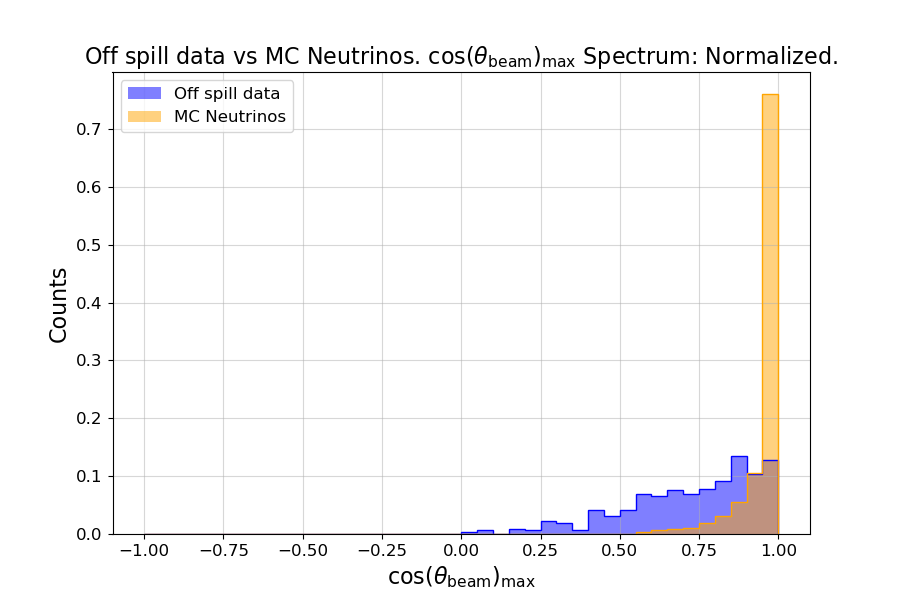
\includegraphics[width=0.32\linewidth]{sections/analysis/Selection/normalized_yes_cuts/sig_bkg_max_directionZ_directionZ2_spectrum_normalized.png}
    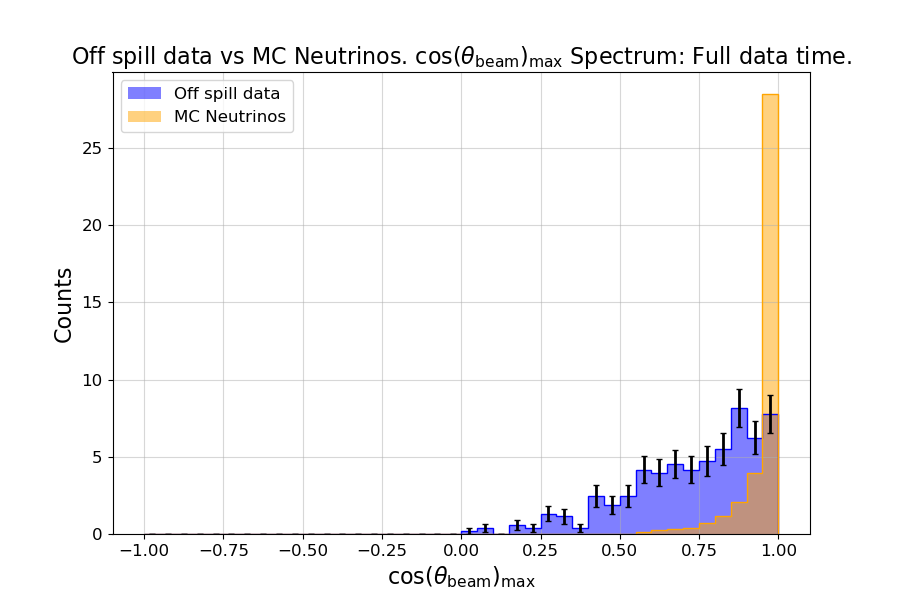
\includegraphics[width=0.32\linewidth]{sections/analysis/Selection/output_test_full_time_yesCut/sig_bkg_max_directionZ_directionZ2_spectrum_full_sig_time.png}
    \caption{Left: $\cos(\theta_{\mathrm{beam}})_{\text{max}}$ distribution before cuts, area normalized to 1. Middle: $\cos(\theta_{\mathrm{beam}})_{\text{max}}$ distribution with all other cuts applied, area normalized to 1. Right: $\cos(\theta_{\mathrm{beam}})_{\text{max}}$ distribution with all other cuts applied, normalized to the expected number of events in the available data.}
    \label{fig:maxZ}
\end{figure}

\begin{figure}[!h]
    \centering
    
\includegraphics[width=0.32\linewidth]{sections/analysis/Selection/output_test_normalized_noCut/sig_bkg_tail_density_normalized.png}
    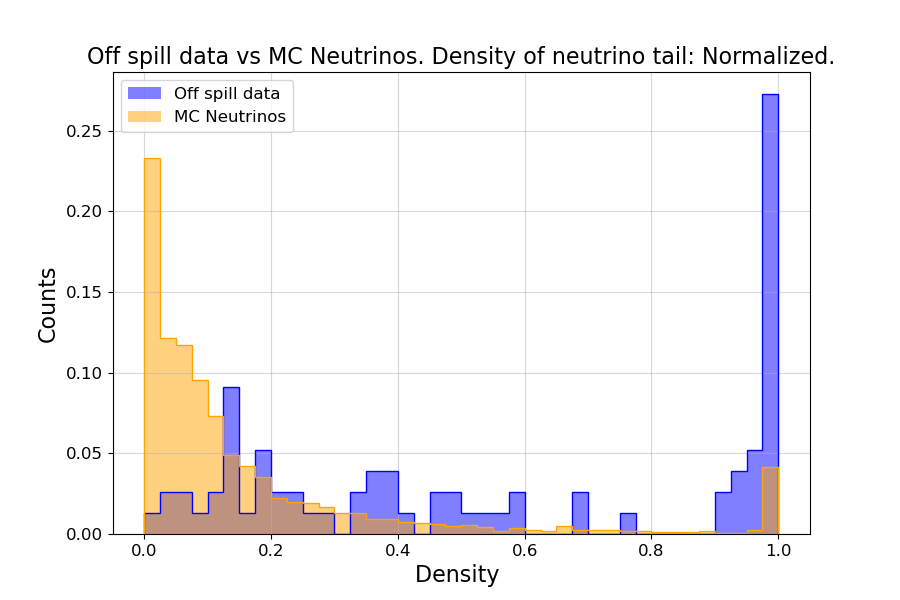
\includegraphics[width=0.32\linewidth]{sections/analysis/Selection/normalized_yes_cuts/sig_bkg_tail_density_normalized.png}
    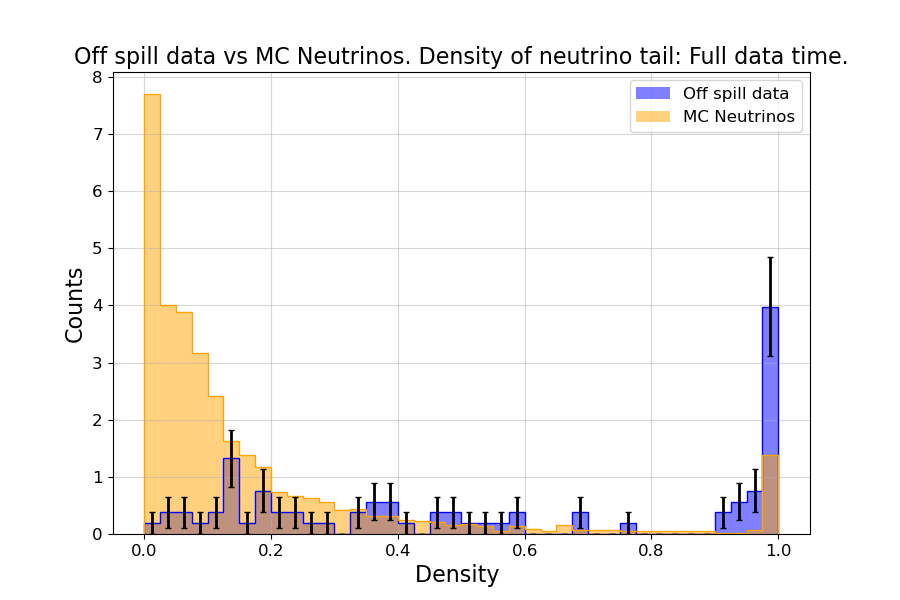
\includegraphics[width=0.32\linewidth]{sections/analysis/Selection/output_test_full_time_yesCut/sig_bkg_tail_density_full_sig_time.png}
    \caption{Left: Tail length density distribution before cuts, area normalized to 1. Middle: Tail length density distribution with all other cuts applied, area normalized to 1. Right: Tail length density distribution with all other cuts applied, normalized to the expected number of events in the available data.}
    \label{fig:tailDensity}
\end{figure}


\begin{figure}[!h]
    \centering
    
\includegraphics[width=0.32\linewidth]{sections/analysis/Selection/output_test_normalized_noCut/sig_bkg_energyDepositedInFifteenth10cm_spectrum_normalized.png}
    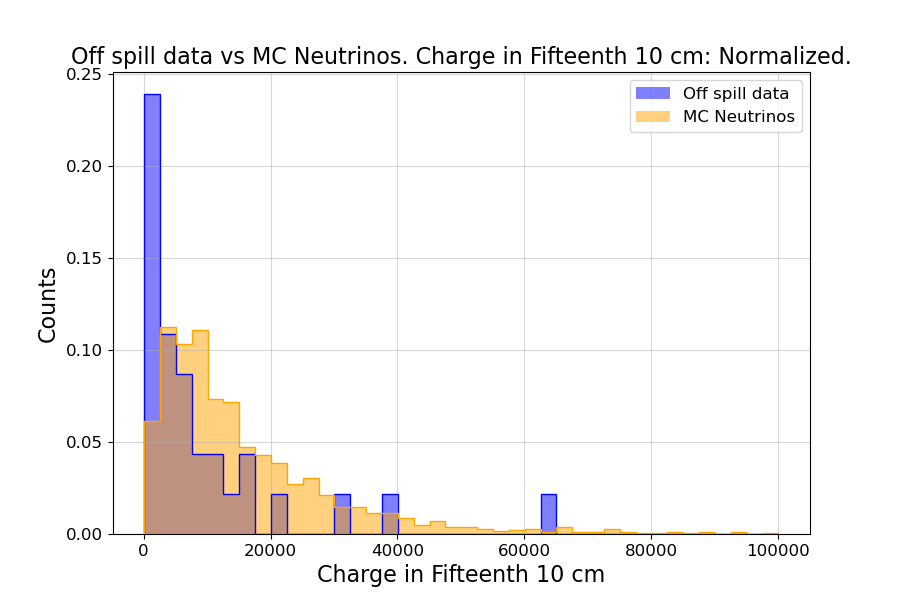
\includegraphics[width=0.32\linewidth]{sections/analysis/Selection/normalized_yes_cuts/sig_bkg_energyDepositedInFifteenth10cm_spectrum_normalized.png}
    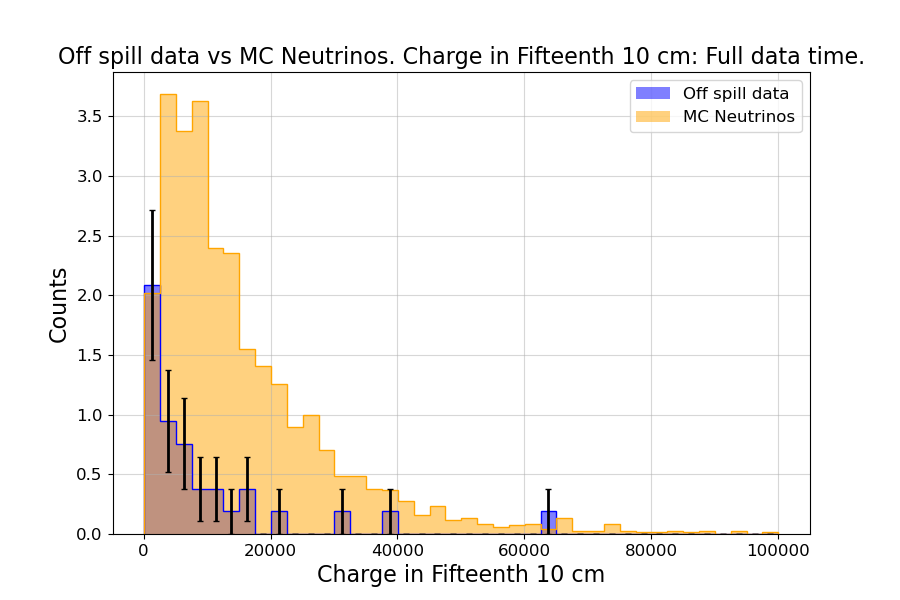
\includegraphics[width=0.32\linewidth]{sections/analysis/Selection/output_test_full_time_yesCut/sig_bkg_energyDepositedInFifteenth10cm_spectrum_full_sig_time.png}
    \caption{Left: Charge in range 140-150 cm from the vertex before cuts, area normalized to 1. Middle: Charge in range 140-150 cm from the vertex with all other cuts applied, area normalized to 1. Right: Charge in range 140-150 cm from the vertex with all other cuts applied, normalized to the expected number of events in the available data.}
    \label{fig:energyFifteenth10}
\end{figure}

\begin{figure}[!h]
    \centering
    
\includegraphics[width=0.32\linewidth]{sections/analysis/Selection/output_test_normalized_noCut/sig_bkg_energyDepositedInFifth10cm_spectrum_normalized.png}
    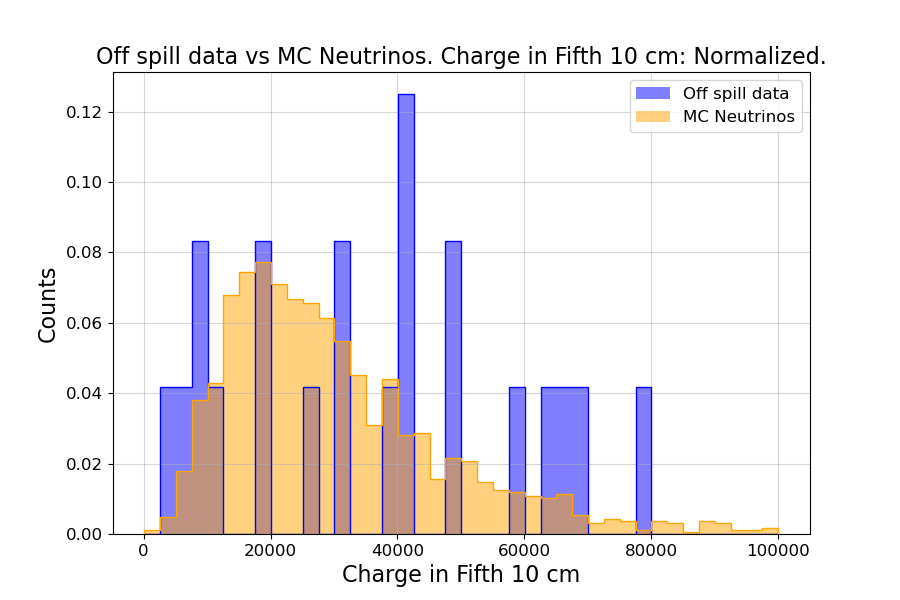
\includegraphics[width=0.32\linewidth]{sections/analysis/Selection/normalized_yes_cuts/sig_bkg_energyDepositedInFifth10cm_spectrum_normalized.png}
    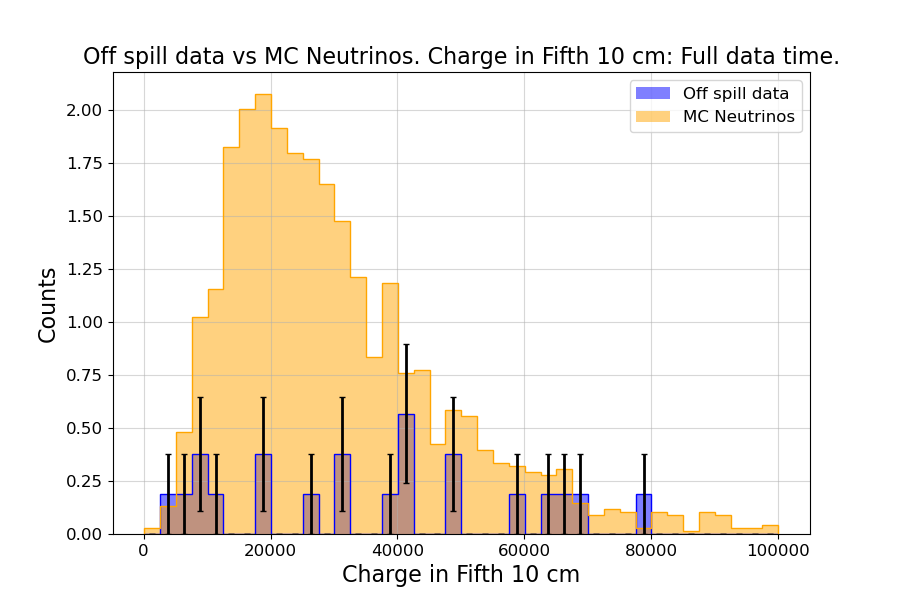
\includegraphics[width=0.32\linewidth]{sections/analysis/Selection/output_test_full_time_yesCut/sig_bkg_energyDepositedInFifth10cm_spectrum_full_sig_time.png}
    \caption{Left: Charge in range 40-50 cm from the vertex before cuts, area normalized to 1. Middle: Charge in range 40-50 cm from the vertex with all other cuts applied, area normalized to 1. Right: Charge in range 40-50 cm from the vertex with all other cuts applied, normalized to the expected number of events in the available data.}
    \label{fig:energyFifth10}
\end{figure}

\begin{figure}[!h]
    \centering
    
\includegraphics[width=0.32\linewidth]{sections/analysis/Selection/output_test_normalized_noCut/sig_bkg_energyDepositedInFirst10cm_spectrum_normalized.png}
    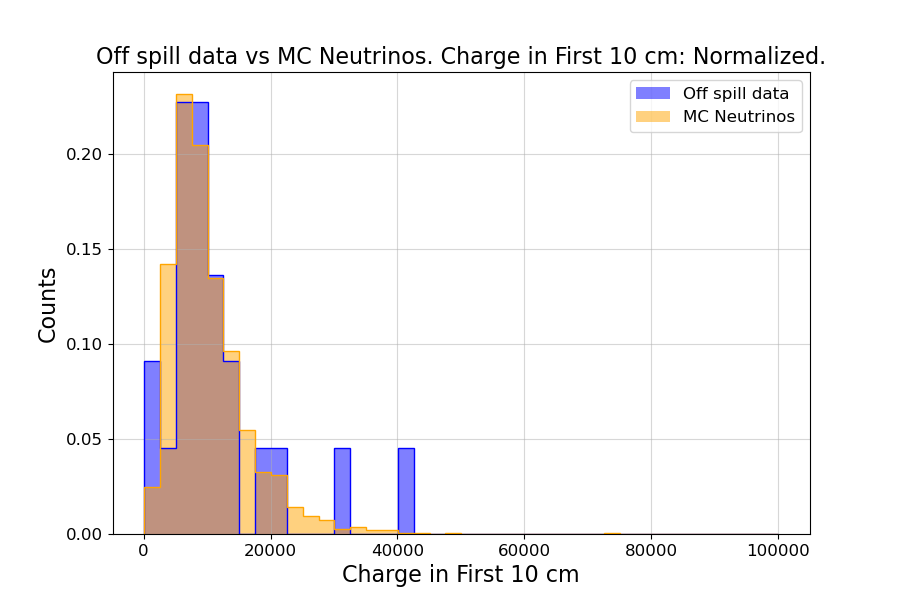
\includegraphics[width=0.32\linewidth]{sections/analysis/Selection/normalized_yes_cuts/sig_bkg_energyDepositedInFirst10cm_spectrum_normalized.png}
    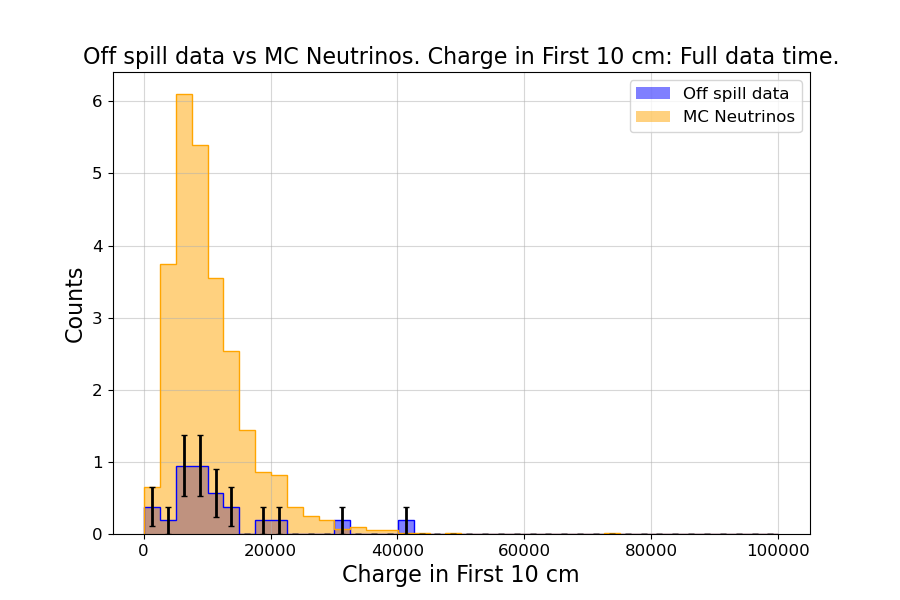
\includegraphics[width=0.32\linewidth]{sections/analysis/Selection/output_test_full_time_yesCut/sig_bkg_energyDepositedInFirst10cm_spectrum_full_sig_time.png}
    \caption{Left: Charge in range 0-10 cm from the vertex before cuts, area normalized to 1. Middle: Charge in range 0-10 cm from the vertex with all other cuts applied, area normalized to 1. Right: Charge in range 0-10 cm from the vertex with all other cuts applied, normalized to the expected number of events in the available data.}
    \label{fig:energyFirst10}
\end{figure}



\begin{figure}[!h]
    \centering
    
\includegraphics[width=0.32\linewidth]{sections/analysis/Selection/output_test_normalized_noCut/sig_bkg_distance_vertexZ_to_ROI_start_normalized.png}
    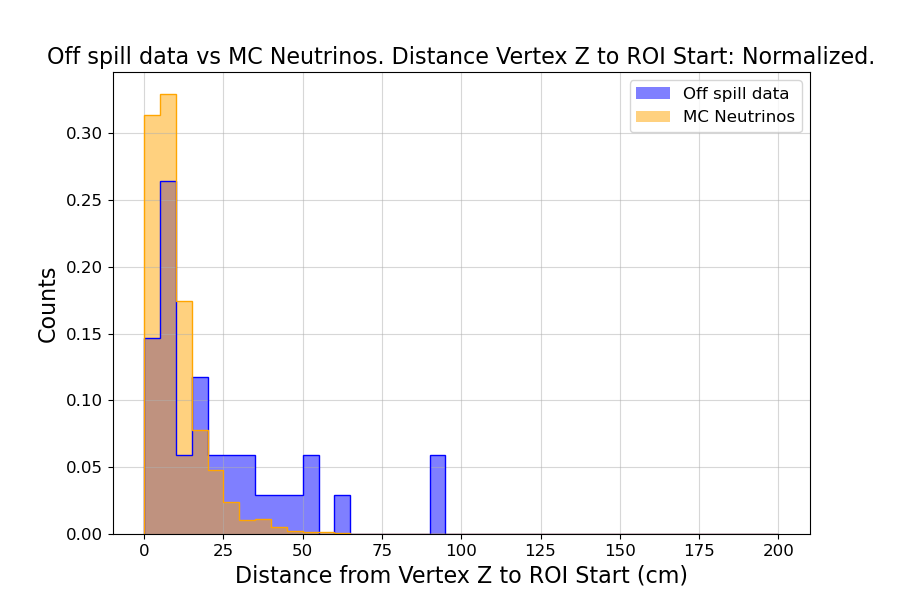
\includegraphics[width=0.32\linewidth]{sections/analysis/Selection/normalized_yes_cuts/sig_bkg_distance_vertexZ_to_ROI_start_normalized.png}
    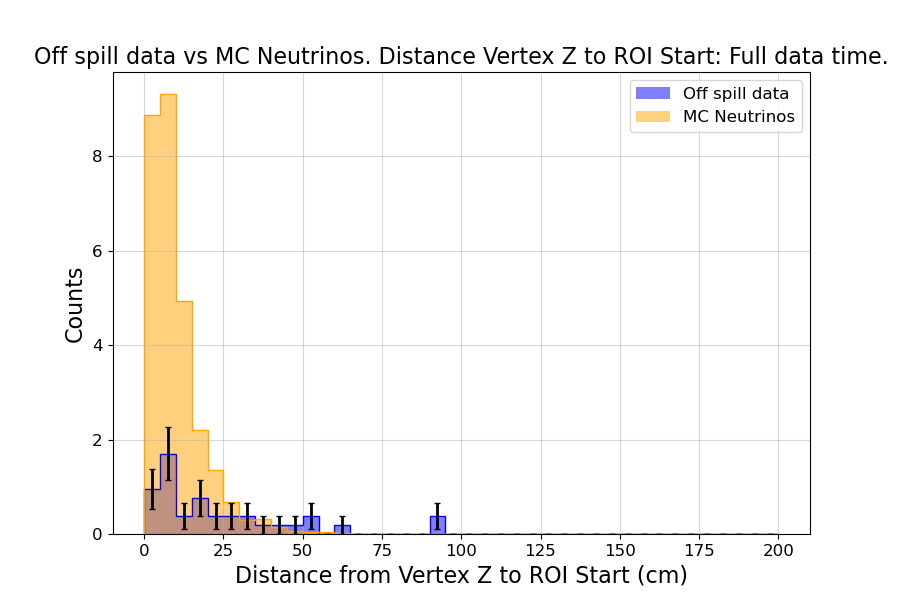
\includegraphics[width=0.32\linewidth]{sections/analysis/Selection/output_test_full_time_yesCut/sig_bkg_distance_vertexZ_to_ROI_start_full_sig_time.png}
    \caption{Left: Distribution of the distance between the vertex Z and the start of the ROI before cuts, area normalized to 1. Middle: Distribution of the distance between the vertex Z and the start of the ROI with all other cuts applied, area normalized to 1. Right: Distribution of the distance between the vertex Z and the start of the ROI with all other cuts applied, normalized to the expected number of events in the available data.}
    \label{fig:ROIdistance}
\end{figure}

\begin{figure}[!h]
    \centering
    
\includegraphics[width=0.32\linewidth]{sections/analysis/Selection/output_test_normalized_noCut/sig_bkg_numberOfPFParticles_spectrum_normalized.png}
    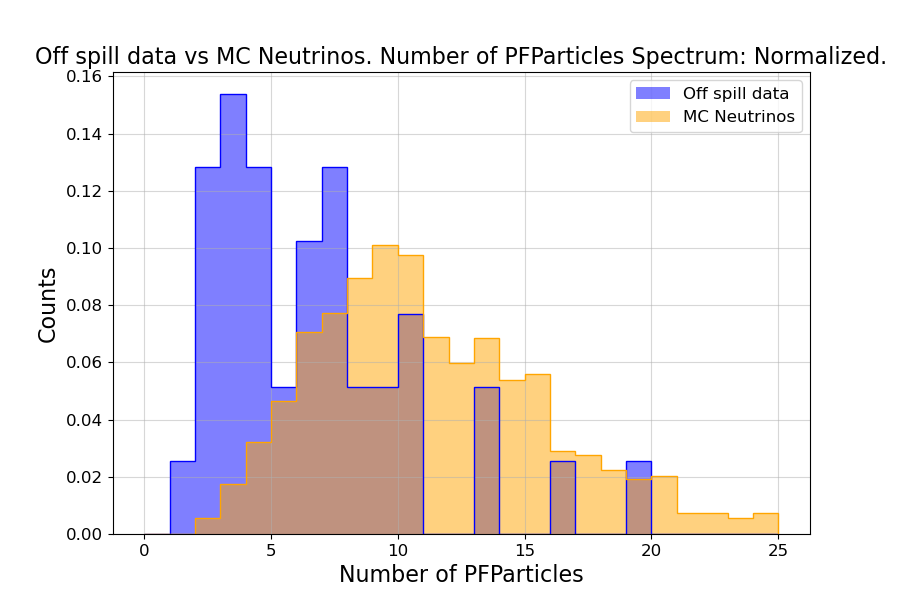
\includegraphics[width=0.32\linewidth]{sections/analysis/Selection/normalized_yes_cuts/sig_bkg_numberOfPFParticles_spectrum_normalized.png}
    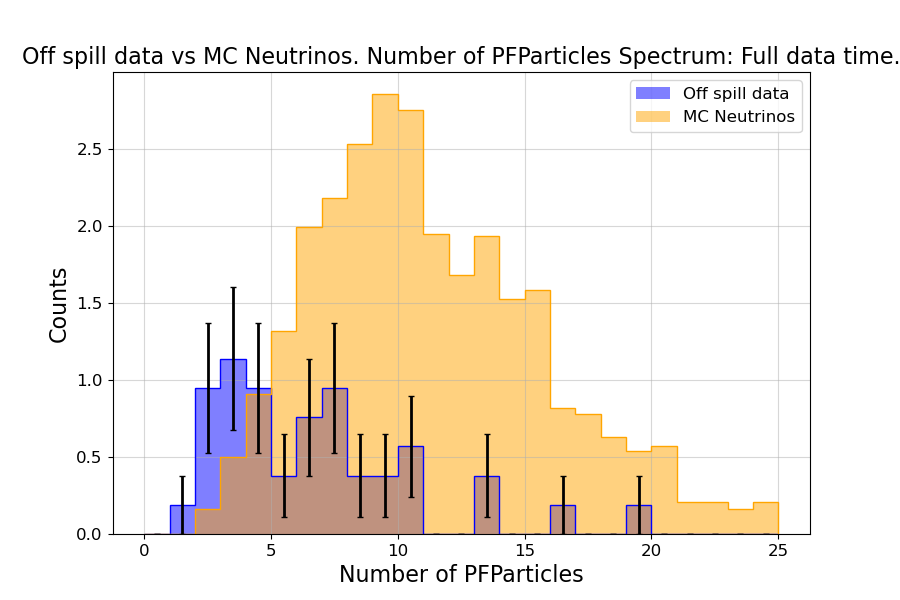
\includegraphics[width=0.32\linewidth]{sections/analysis/Selection/output_test_full_time_yesCut/sig_bkg_numberOfPFParticles_spectrum_full_sig_time.png}
    \caption{Left: Number of daughter particles before cuts, area normalized to 1. Middle: Number of daughter particles with all other cuts applied, area normalized to 1. Right: Number of daughter particles with all other cuts applied, normalized to the expected number of events in the available data.}
    \label{fig:nPFPs}
\end{figure}



\begin{figure}[!h]
    \centering
    
\includegraphics[width=0.32\linewidth]{sections/analysis/Selection/output_test_normalized_noCut/sig_bkg_vertexZ_spectrum_normalized.png}
    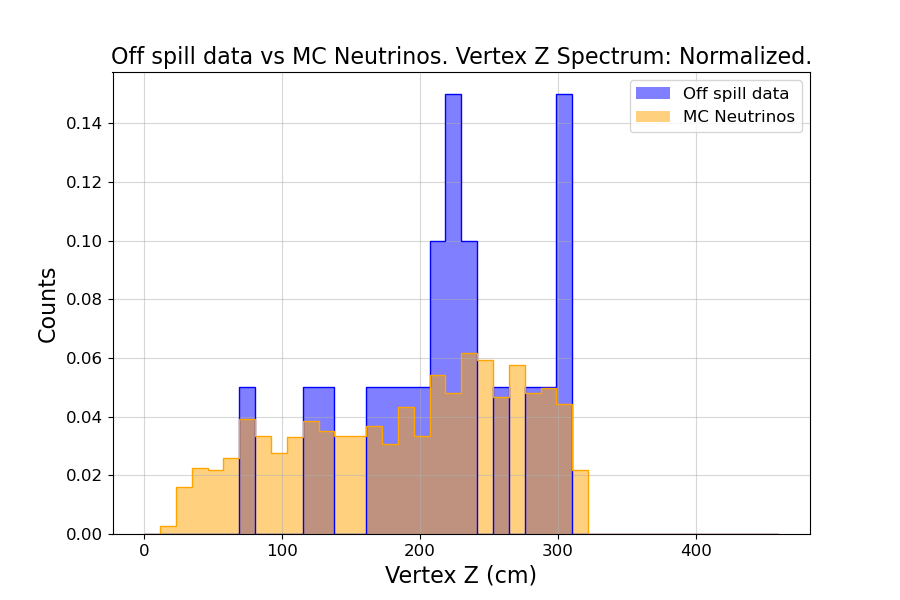
\includegraphics[width=0.32\linewidth]{sections/analysis/Selection/normalized_yes_cuts/sig_bkg_vertexZ_spectrum_normalized.png}
    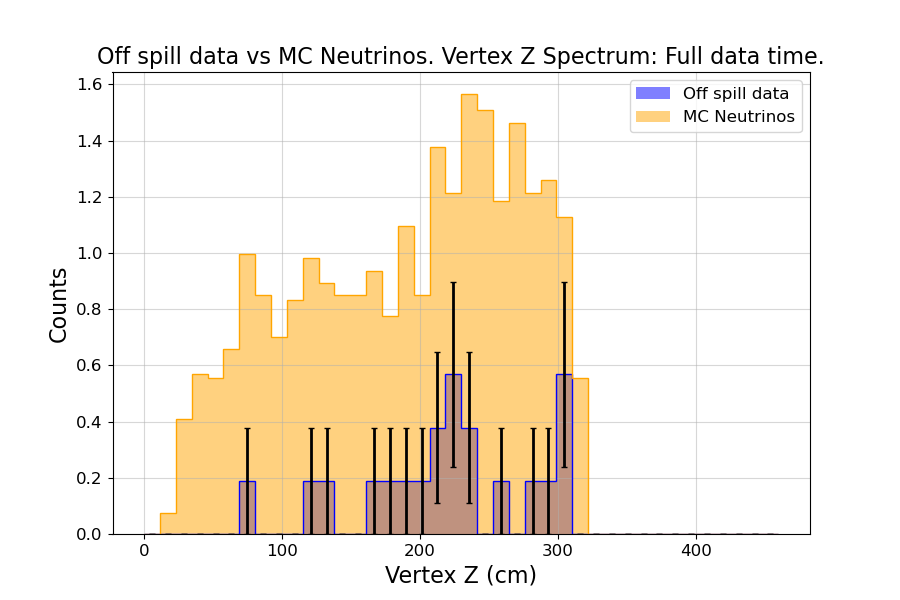
\includegraphics[width=0.32\linewidth]{sections/analysis/Selection/output_test_full_time_yesCut/sig_bkg_vertexZ_spectrum_full_sig_time.png}
    \caption{Left: Vertex position in Z before cuts, area normalized to 1. Middle: Vertex position in Z with all other cuts applied, area normalized to 1. Right: Vertex position in Z with all other cuts applied, normalized to the expected number of events in the available data.}
    \label{fig:vertexZ}
\end{figure}

\begin{figure}[!h]
    \centering
    
\includegraphics[width=0.32\linewidth]{sections/analysis/Selection/output_test_normalized_noCut/sig_bkg_vertexY_spectrum_normalized.png}
    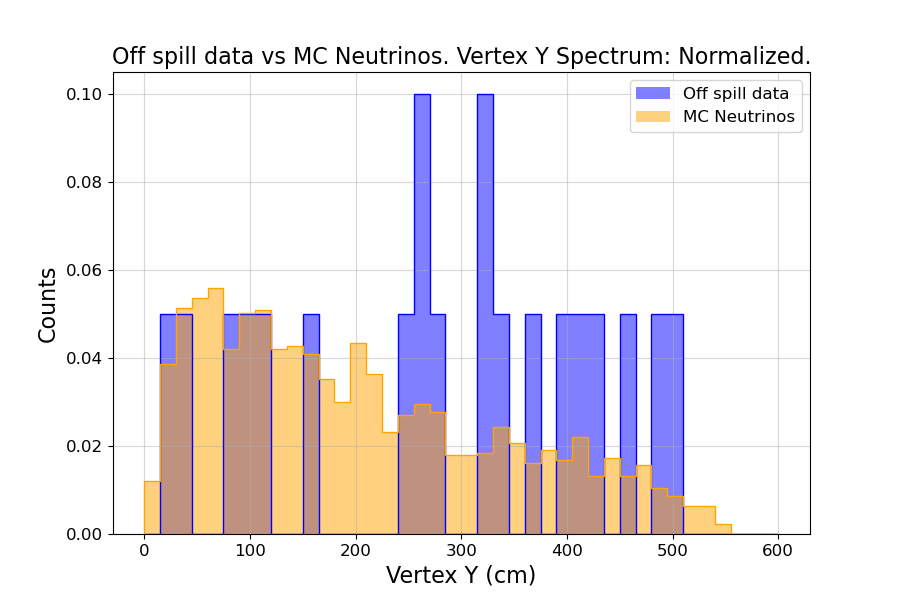
\includegraphics[width=0.32\linewidth]{sections/analysis/Selection/normalized_yes_cuts/sig_bkg_vertexY_spectrum_normalized.png}
    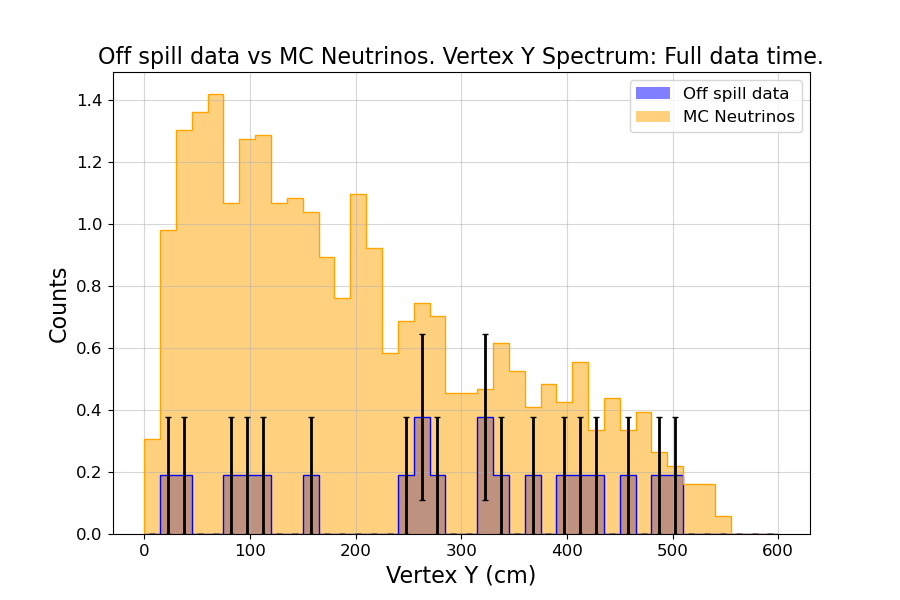
\includegraphics[width=0.32\linewidth]{sections/analysis/Selection/output_test_full_time_yesCut/sig_bkg_vertexY_spectrum_full_sig_time.png}
    \caption{Left: Vertex position in Y before cuts, area normalized to 1. Middle: Vertex position in Y with all other cuts applied, area normalized to 1. Right: Vertex position in Y with all other cuts applied, normalized to the expected number of events in the available data.}
    \label{fig:vertexY}
\end{figure}


\begin{figure}[!h]
    \centering
    
\includegraphics[width=0.32\linewidth]{sections/analysis/Selection/output_test_normalized_noCut/sig_bkg_ROI_Z_size_spectrum_normalized.png}
    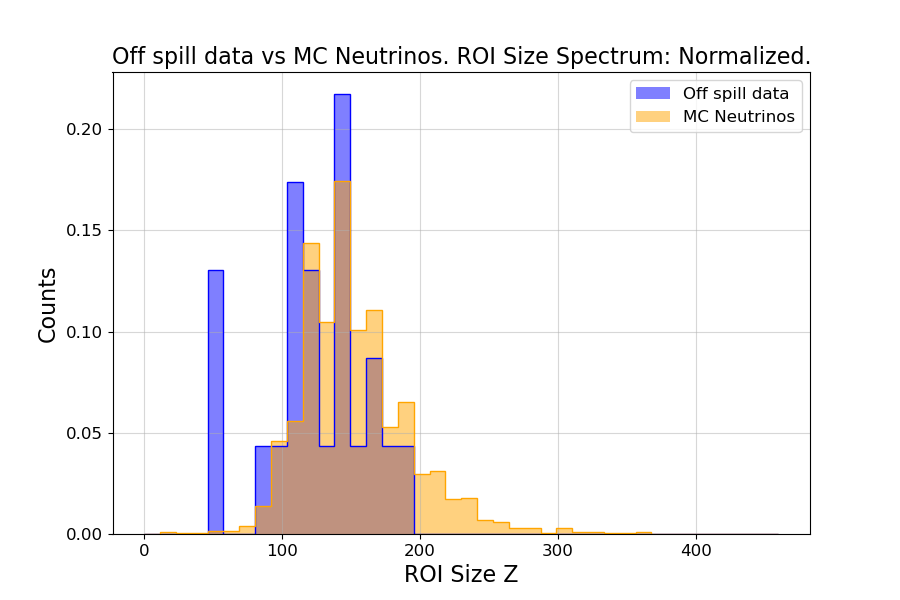
\includegraphics[width=0.32\linewidth]{sections/analysis/Selection/normalized_yes_cuts/sig_bkg_ROI_Z_size_spectrum_normalized.png}
    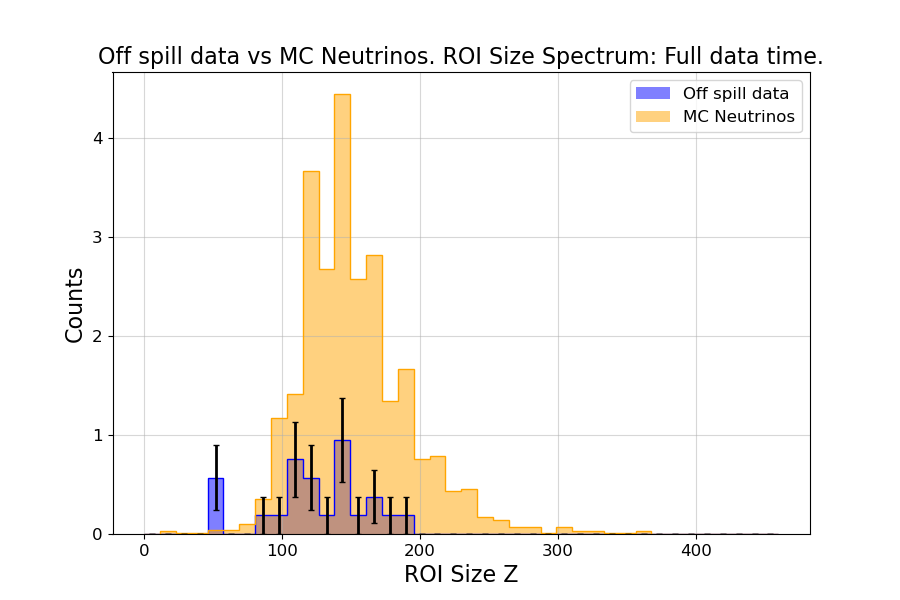
\includegraphics[width=0.32\linewidth]{sections/analysis/Selection/output_test_full_time_yesCut/sig_bkg_ROI_Z_size_spectrum_full_sig_time.png}
    \caption{Left: ROI size distribution before cuts, area normalized to 1. Middle: ROI size distribution  with all other cuts applied, area normalized to 1. Right: ROI size distribution with all other cuts applied, normalized to the expected number of events in the available data.}
    \label{fig:ROIsize}
\end{figure}







 